\documentclass[11pt]{article}\usepackage[margin=1in]{geometry}\usepackage{amsmath,amssymb,amsthm,mathtools}\usepackage{graphicx}\graphicspath{{figures/}{../figures/}{figs/}{./}}\usepackage{enumitem}\usepackage{hyperref}\usepackage{cleveref}\usepackage{tikz}\usetikzlibrary{arrows.meta,positioning,calc,shapes.geometric}\usepackage{float}\usepackage{rotating}\usepackage[most]{tcolorbox}\usepackage{kotex}\usepackage{booktabs}\emergencystretch=1.6em\tolerance=2000 \crefname{assumption}{Assumption}{Assumptions}\Crefname{assumption}{Assumption}{Assumptions}\crefname{definition}{Definition}{Definitions}\Crefname{definition}{Definition}{Definitions}\crefname{proposition}{Proposition}{Propositions}\Crefname{proposition}{Proposition}{Propositions}\crefname{fact}{Fact}{Facts}\Crefname{fact}{Fact}{Facts} \newtheorem{assumption}{Assumption}\newtheorem{definition}{Definition}\newtheorem{lemma}{Lemma}\newtheorem{proposition}{Proposition}\newtheorem{theorem}{Theorem}\newtheorem{corollary}{Corollary}\newtheorem{fact}{Fact}\theoremstyle{remark}\newtheorem{remark}{Remark} \newcommand{\R}{\mathbb{R}}\newcommand{\xb}{\bar x}\newcommand{\Ab}{\bar A}\newcommand{\By}{\bar B_y}\newcommand{\U}{\mathcal U}\newcommand{\Z}{\mathcal Z}
\newcommand{\Cset}{\mathcal C}\newcommand{\Pcl}{\mathcal P}\newcommand{\Kset}{\mathcal K}

\title{적응 철학이 내재된 RL policy:\\ 문제 정의와 사양}
\author{Junhyeok Yoon}
\date{2026년 11월 12일 (개정 3, v2 설계의 기록: 중단됨)}

\begin{document}
\maketitle

\begin{abstract}
Instance model 없이 class 수준 구조만 아는 control-affine system에서, 내부 상태가 배치 중 적응하는 신경망 policy를 RL로 학습하는 문제를 정의한다. 요구는 학습 결과와 무관하게, 즉 모든 weight와 모든 RL action에서 state 제약, input 제약, 실행 가능성이 구조로 성립하는 것이다. Policy는 task policy, command interface, adaptive core의 세 부분으로 이루어지고, 명령은 reference와 허용 오차의 쌍이다. Adaptive core는 명령된 허용 오차 안에 오차를 유지하며, command interface는 오차와 제약의 여유에 따라 reference의 진행과 허용 오차의 수축을 늦춘다. 아래층은 여유, saturation의 작동, 제안과 실현의 차이를 측정값으로 보고하고, 무엇이 실현 가능한지는 task policy가 이 보고를 통해 학습한다. 학습은 세 부분이 결합된 loop에서만 이루어진다. 이 문서는 대상, 구조, 신호, 요구 사항, 가정, 계약, 평가 기준을 정하고, 각 항목이 증명되었는지 부분 확인인지 미해결인지를 구분한다. \Cref{sec:prelim}은 passivity와 port-Hamiltonian system을 정의하고, \Cref{sec:policy}는 adaptive core가 고전 적응 법칙의 passive 연결을 일반화한 것임을 증명과 함께 보인다. 제약 보장의 유도는 별도 노트에 있다. 학습 비교는 또 다른 노트에 있으며, 사전에 정한 규칙에 따라 이 설계는 중단되었다.
\end{abstract}

\section{Overview}
\label{sec:overview}

\Cref{fig:arch}는 policy의 세 부분과 주고받는 신호를, \Cref{fig:chain}은 보장이 닫히는 순서를 보인다. \Cref{fig:chain}에서 초록색은 모든 weight와 모든 action에서 구조로 성립해야 하는 단계, 주황색은 class 조건을 쓰는 단계이고, 점선 테두리는 상대 차수 2에서 아직 유도하지 않은 단계이다. 상대 차수 1에서는 위 네 단계가 별도 노트에서 증명되었다.

\begin{figure}[H]
\centering
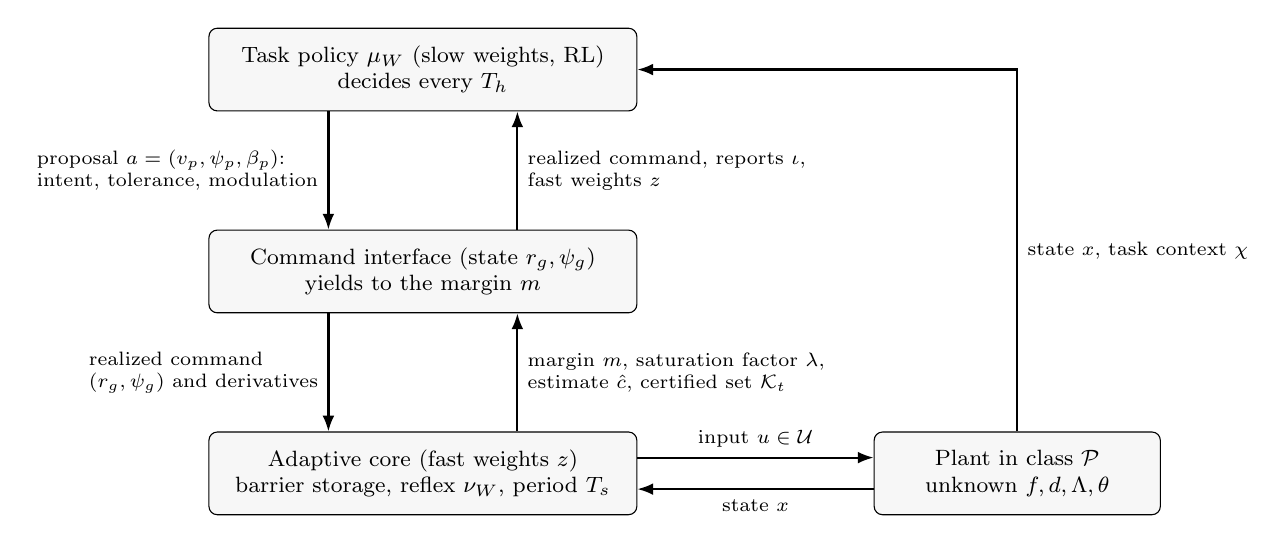
\begin{tikzpicture}[
  every node/.style={font=\footnotesize, align=center},
  blk/.style={draw, rounded corners=3pt, minimum height=1.05cm, text width=5.2cm, fill=gray!6},
  arr/.style={-{Latex[length=2mm]}, thick},
  lab/.style={font=\scriptsize, align=left}]
\node[blk] (mu) {Task policy $\mu_W$ (slow weights, RL)\\ decides every $T_h$};
\node[blk, below=1.5cm of mu] (gov) {Command interface (state $r_g,\psi_g$)\\ yields to the margin $m$};
\node[blk, below=1.5cm of gov] (core) {Adaptive core (fast weights $z$)\\ barrier storage, reflex $\nu_W$, period $T_s$};
\node[blk, right=3.0cm of core, text width=3.4cm] (plant) {Plant in class $\mathcal P$\\ unknown $f,d,\Lambda,\theta$};
\draw[arr] ([xshift=-1.2cm]mu.south) -- node[lab, left]{proposal $a=(v_p,\psi_p,\beta_p)$:\\ intent, tolerance, modulation} ([xshift=-1.2cm]gov.north);
\draw[arr] ([xshift=1.2cm]gov.north) -- node[lab, right]{realized command, reports $\iota$,\\ fast weights $z$} ([xshift=1.2cm]mu.south);
\draw[arr] ([xshift=-1.2cm]gov.south) -- node[lab, left]{realized command\\ $(r_g,\psi_g)$ and derivatives} ([xshift=-1.2cm]core.north);
\draw[arr] ([xshift=1.2cm]core.north) -- node[lab, right]{margin $m$, saturation factor $\lambda$,\\ estimate $\hat c$, certified set $\mathcal K_t$} ([xshift=1.2cm]gov.south);
\draw[arr] ([yshift=0.2cm]core.east) -- node[lab, above]{input $u\in\mathcal U$} ([yshift=0.2cm]plant.west);
\draw[arr] ([yshift=-0.2cm]plant.west) -- node[lab, below]{state $x$} ([yshift=-0.2cm]core.east);
\draw[arr] (plant.north) |- node[lab, pos=0.25, right]{state $x$, task context $\chi$} (mu.east);
\end{tikzpicture}
\caption{Policy architecture and exchanged signals}
\label{fig:arch}
\end{figure}

\begin{figure}[H]
\centering
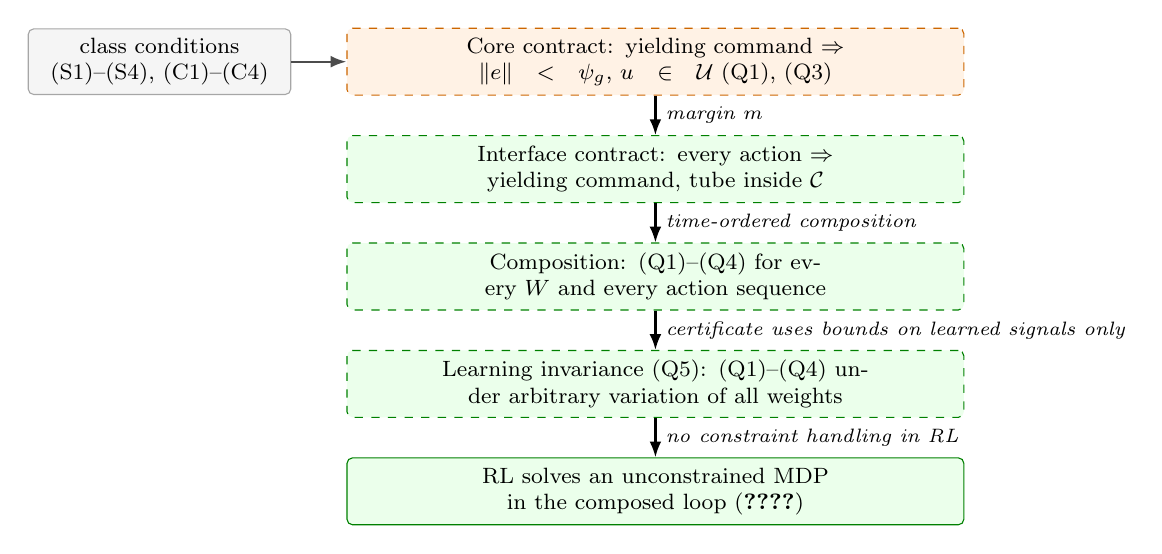
\begin{tikzpicture}[
  node distance=0.5cm and 0.7cm,
  every node/.style={font=\footnotesize, align=center},
  unc/.style={draw=green!50!black, fill=green!8, rounded corners=2pt, text width=7.6cm, minimum height=0.85cm},
  con/.style={draw=orange!80!black, fill=orange!10, rounded corners=2pt, text width=7.6cm, minimum height=0.85cm},
  feed/.style={draw=gray!70, fill=gray!8, rounded corners=2pt, text width=3.1cm, minimum height=0.8cm},
  arr/.style={-{Latex[length=2mm]}, thick},
  lab/.style={font=\scriptsize\itshape, align=left}]
\node[con, dashed] (n1) {Core contract: yielding command $\Rightarrow$ $\|e\|<\psi_g$, $u\in\mathcal U$ (Q1), (Q3)};
\node[unc, dashed, below=of n1] (n2) {Interface contract: every action $\Rightarrow$ yielding command, tube inside $\mathcal C$};
\node[unc, dashed, below=of n2] (n3) {Composition: (Q1)--(Q4) for every $W$ and every action sequence};
\node[unc, dashed, below=of n3] (n4) {Learning invariance (Q5): (Q1)--(Q4) under arbitrary variation of all weights};
\node[unc, below=of n4] (n5) {RL solves an unconstrained MDP in the composed loop (\Cref{def:mdp,def:learn})};
\draw[arr] (n1) -- node[lab, right]{margin $m$} (n2);
\draw[arr] (n2) -- node[lab, right]{time-ordered composition} (n3);
\draw[arr] (n3) -- node[lab, right]{certificate uses bounds on learned signals only} (n4);
\draw[arr] (n4) -- node[lab, right]{no constraint handling in RL} (n5);
\node[feed, left=of n1] (a1) {class conditions\\ (S1)--(S4), (C1)--(C4)};
\draw[arr, gray!60!black] (a1) -- (n1);
\end{tikzpicture}
\caption{Closure order of the guarantees}
\label{fig:chain}
\end{figure}

\section{범위와 원칙}
\label{sec:scope}

\textbf{직관 (역할의 분배).} 손으로 문 손잡이를 잡을 때 뇌는 손을 대략 어디로 보낼지만 정하고, 손잡이 모양에 맞추는 일은 손이 자신의 감각으로 처리한다. 이것이 가능한 것은 뇌가 손이 무엇을 해 주는지를 알고, 손이 명령에 여유가 있음을 알기 때문이다. 이 문서의 구조는 이 분배를 세 가지 형식 요소로 옮긴다: 명령은 의도와 허용 오차의 쌍이고, 아래층은 허용 오차 안에서 자율적이며, 두 층이 서로에게 요구하고 보장하는 것은 계약으로 명시된다.

\textbf{목표.} 대상은 로봇 전용 제어기가 아니라, 적응 제어의 철학이 구조에 들어 있는 RL policy이다. 로봇은 적용 대상이며, policy는 중력 항이나 regressor 같은 instance model을 포함하지 않는다.

\textbf{설계 원칙.}
\begin{itemize}
\item \textbf{구조에 의한 보장.} 보장은 학습이 잘 되었을 때만 성립하는 것이 아니라 모든 weight에서 성립한다. 학습 품질은 성능에만 영향을 준다.
\item \textbf{두 수준의 certainty equivalence.} Task policy는 아래층이 보고한 측정값과 추정치를 참으로 두고 행동하고, core는 명령을 참인 의도로 두고 행동한다. 각 수준은 자신의 불확실성만 다룬다.
\item \textbf{오차로 구동되는 세 시간 척도의 적응.} Fast weight는 변환된 추종 오차로, command interface는 여유로, slow weight는 task reward로 갱신된다.
\item \textbf{협력에 의한 경계.} 추종 오차의 경계는 위층을 적대적으로 가정한 최악 경우에서 계산하지 않고, 명령으로 지정되며 위층이 양보한다.
\item \textbf{학습 중의 결합.} 학습은 세 부분이 결합된 loop에서만 이루어지고, 아래층의 상태와 보고는 학습자에게 숨겨지지 않는다. 아래층이 무엇을 할 수 있는지는 미리 계산해 넘겨주지 않고, task policy가 측정된 보고를 통해 학습한다.
\item \textbf{결합의 기준.} 한 요소는 다른 요소의 제한 가정을 제거할 때만 포함한다. 제어 loop의 차수와 tick당 계산량은 표준 recurrent 신경망 policy의 수준을 넘지 않는다.
\end{itemize}

\textbf{범위 밖.} Output feedback, 입력 방향을 모르는 system, 확률적 보장, hardware 실험은 이 사양에 포함하지 않는다.

\section{System class와 제약}
\label{sec:plant}

\begin{definition}[Plant class]
\label{def:plant}
The class $\Pcl$ consists of the systems
\begin{equation}
\dot x=f(x,\theta)+g_0(x)\,\Lambda(x,\theta)\,\big(u+d(x,\theta,t)\big),\qquad \eta:=c(x),
\label{eq:plant}
\end{equation}
with state $x\in\R^n$, input $u\in\R^m$, controlled output $\eta\in\R^m$ and unknown parameter $\theta$, that satisfy:
\begin{itemize}
\item[\textbf{(S1)}] (Measured state, known structure) $x$ is measured; $g_0$ and $c$ are known; $f$, $d$, $\Lambda$ and $\theta$ are unknown; $\theta\in\Theta$ with $\Theta$ compact.
\item[\textbf{(S2)}] (Relative degree and input gain) $\eta$ has a uniform relative degree $\varrho\in\{1,2\}$ with respect to $u$, and the high-frequency gain $\Gamma(x,\theta)\in\R^{m\times m}$ satisfies $w^\top\Gamma(x,\theta)\,w\ge\gamma_0\|w\|^2$ $\forall w\in\R^m$ and $\|\Gamma(x,\theta)\|\le\gamma_1$ for known constants $0<\gamma_0\le\gamma_1$.
\item[\textbf{(S3)}] (Internal dynamics) If $n>\varrho m$, the internal dynamics are bounded-input bounded-state with respect to $(\eta,\dots,\eta^{(\varrho-1)})$.
\item[\textbf{(S4)}] (Envelopes) Known continuous functions $\bar F$ and $\bar d$ bound the drift of $\eta^{(\varrho)}$ and the disturbance on the constraint region, uniformly in $\theta\in\Theta$.
\end{itemize}
\end{definition}

\begin{remark}[Mechanical systems]
\label{rem:mech}
$n_q$자유도 기계 system $M(q)\ddot q+C(q,\dot q)\dot q+g(q)+F\dot q=\tau$에서 $x=(q,\dot q)$, $\eta=q$, $u=\tau$로 두면 $\varrho=2$이고 high-frequency gain은 관성 행렬의 역이다.
\[
\Gamma(x,\theta)=M(q)^{-1}.
\]
(S2)는 $M(q)$의 고유값 범위만을, (S4)는 Coriolis, 중력, 마찰 항의 크기 상한만을 요구하며, 그 함수 형태는 요구하지 않는다.
\end{remark}

\begin{definition}[Constraints]
\label{def:constraints}
\begin{itemize}
\item State constraint: $\Cset:=\{\eta\in\R^m:\ h_j(\eta)\ge0,\ j=1,\dots,p\}$ with known $h_j\in C^2$, $\Cset$ compact with nonempty interior.
\item Input constraint: $\U:=\{u\in\R^m:\ |u_i|\le\bar u_i,\ i=1,\dots,m\}$ with known $\bar u_i>0$.
\end{itemize}
\end{definition}

\begin{definition}[Task]
\label{def:task}
A task is a pair $(\chi,\theta)$ with observed context $\chi\sim\mathcal D_\chi$ and hidden parameter $\theta\sim\mathcal D_\theta$, $\operatorname{supp}\mathcal D_\theta\subseteq\Theta$, together with a reward rate $R(x,u,\chi)$.
\end{definition}

\section{준비: passivity와 port-Hamiltonian system}
\label{sec:prelim}

\textbf{직관 (에너지 장부).} Passivity는 system 안에 에너지원이 없다는 성질을 입출력으로 표현한 것이다. 저장된 에너지는 입출력 port로 들어온 일률만큼만 늘 수 있고, 나머지는 소산된다. 이 성질은 연결에 대해 닫혀 있어서, passive한 두 system을 음의 feedback으로 연결하면 두 storage의 합이 늘지 않는다. 고전 적응 제어의 안정성 증명은 이 연결의 한 예이고(\Cref{lem:classical}), adaptive core는 그 연결에서 적응 쪽 block을 학습되는 port-Hamiltonian system으로 바꾼 것이다(\Cref{lem:corepH}).

\begin{definition}[Passivity]
\label{def:passive}
Consider a system with state $x\in\R^{n}$, input $u\in\R^{m}$ and output $y\in\R^{m}$,
\[
\dot x=f(x,u,t),\qquad y=h(x,u,t).
\]
\begin{itemize}
\item A \textbf{\emph{storage}} is a $C^1$ function $S:\R^n\to\R_{\ge0}$.
\item The system is \textbf{\emph{passive}} with storage $S$ if, along every solution and for every input,
\[
\dot S\le u^\top y .
\]
\item It is \textbf{\emph{lossless}} if equality holds, and \textbf{\emph{output strictly passive}} if $\exists\,\varepsilon>0$ with $\dot S\le u^\top y-\varepsilon\|y\|^2$.
\end{itemize}
\end{definition}

\begin{lemma}[Negative feedback interconnection]
\label{lem:interconnect}
Let $\Sigma_1$, $\Sigma_2$ be passive with storages $S_1$, $S_2$, inputs $u_1,u_2\in\R^m$ and outputs $y_1,y_2\in\R^m$, connected by $u_1=-y_2$ and $u_2=y_1$. Then $S_1+S_2$ is nonincreasing along every solution of the interconnection.
\end{lemma}

\begin{proof}
두 부등식을 더한다.
\[
\dot S_1+\dot S_2\le u_1^\top y_1+u_2^\top y_2 .
\]
연결식을 넣는다.
\[
u_1^\top y_1+u_2^\top y_2=-y_2^\top y_1+y_1^\top y_2=0 .
\]
\end{proof}

\begin{definition}[Port-Hamiltonian system]
\label{def:ph}
A \textbf{\emph{port-Hamiltonian system}} with state $z\in\R^{n}$ and port $(u,y)\in\R^m\times\R^m$ is
\[
\dot z=\big(\mathcal J(z,t)-\mathcal R(z,t)\big)\nabla H(z)+\mathcal G(z,t)\,u,\qquad y=\mathcal G(z,t)^\top\nabla H(z),
\]
where
\begin{itemize}
\item the \textbf{\emph{Hamiltonian}} $H:\R^n\to\R$ is $C^1$ and bounded from below;
\item the \textbf{\emph{interconnection}} $\mathcal J(z,t)\in\R^{n\times n}$ satisfies $\mathcal J=-\mathcal J^\top$;
\item the \textbf{\emph{dissipation}} $\mathcal R(z,t)\in\R^{n\times n}$ satisfies $\mathcal R=\mathcal R^\top\succeq0$;
\item the \textbf{\emph{port matrix}} is $\mathcal G(z,t)\in\R^{n\times m}$.
\end{itemize}
\end{definition}

\begin{lemma}[Port-Hamiltonian systems are passive]
\label{lem:phpassive}
For every $\mathcal J$, $\mathcal R$, $\mathcal G$ satisfying the conditions of \Cref{def:ph}, including time-varying ones,
\[
\dot H=-\nabla H^\top\mathcal R\,\nabla H+u^\top y\le u^\top y ,
\]
so the system is passive with storage $H-\inf H$.
\end{lemma}

\begin{proof}
해를 $z(t)$로 두고, 각 시각의 gradient를 벡터 하나로 부른다.
\[
v(t):=\nabla H\big(z(t)\big)\in\R^n .
\]
$H\in C^1$이고 $z(t)$가 미분 가능한 시각에서 연쇄 법칙이 성립한다.
\[
\frac{d}{dt}H\big(z(t)\big)=v^\top\dot z .
\]
$\dot z$에 \Cref{def:ph}의 우변을 넣는다. 우변이 $\nabla H$로 만들어져 있으므로 결과는 $v$만의 식이다.
\[
\dot H=v^\top\mathcal J\,v-v^\top\mathcal R\,v+v^\top\mathcal G\,u .
\]
세 항을 각각 정리한다. 각 단계는 $v$가 어떤 벡터이든 성립하므로 $H$의 구체적인 형태를 쓰지 않는다. 첫째 항은 scalar가 자기 transpose와 같다는 것과 $\mathcal J^\top=-\mathcal J$에서 0이다.
\[
v^\top\mathcal J\,v=\big(v^\top\mathcal J\,v\big)^\top=v^\top\mathcal J^\top v=-v^\top\mathcal J\,v\ \Longrightarrow\ v^\top\mathcal J\,v=0 .
\]
둘째 항은 $\mathcal R$의 정의에서 0 이상이다.
\[
\mathcal R\succeq0\ \Longrightarrow\ v^\top\mathcal R\,v\ge0 .
\]
셋째 항은 출력의 정의이다.
\[
v^\top\mathcal G\,u=\big(\mathcal G^\top v\big)^\top u=y^\top u .
\]
\end{proof}

\begin{remark}[Why no formula for $H$ is needed]
\label{rem:noformula}
일반적인 ODE $\dot z=f(z)$에서는 $\dot H=\nabla H^\top f$가 $H$와 $f$ 모두에 의존한다. Port-Hamiltonian system에서는 vector field 자체를 $\nabla H$로 만들기 때문에, $\dot H$가 $\nabla H$의 2차식과 port 항으로 바뀌고 그 부호는 $\mathcal J$와 $\mathcal R$의 구조만으로 정해진다. 기하적으로 $\mathcal J\nabla H$는 $\nabla H$와 직교하므로 $H$의 등위면을 따라 움직이고, $-\mathcal R\nabla H$는 $H$가 줄어드는 방향이다.
\[
\nabla H^\top\big(\mathcal J\nabla H\big)=0,\qquad \nabla H^\top\big(-\mathcal R\nabla H\big)\le0 .
\]
2차 Hamiltonian $H(z)=\tfrac12z^\top Qz$($Q\succ0$)에서는 $\nabla H=Qz$이고, 같은 계산이 다음과 같다.
\[
\dot z=(\mathcal J-\mathcal R)Qz+\mathcal Gu,\qquad \dot H=z^\top Q\dot z=-(Qz)^\top\mathcal R\,(Qz)+(\mathcal G^\top Qz)^\top u .
\]
\Cref{def:hclass}의 $H_W$에서는 \Cref{fact:hclass}의 gradient를 $v$에 넣으면 같은 결론이 나온다. 계산에 쓰인 $H$의 성질은 $C^1$뿐이다. Bounded below는 $H-\inf H\ge0$을 storage로 쓰기 위해서만 필요하고, 해의 존재는 $\nabla H$가 locally Lipschitz일 때 보장된다.
\end{remark}

\textbf{직관 (이름과 세 구조).} 이름의 Hamiltonian은 해석역학에서 운동이 에너지 함수의 gradient와 skew 구조로 생성된다는 것($\dot z=\mathcal J\nabla H$이면 $H$가 보존된다)에서, port는 곱이 일률이 되는 입출력 쌍에서 왔다(Maschke와 van der Schaft, 1992). $\mathcal J$는 상태 사이에서 에너지를 옮기기만 하고, $\mathcal R$은 없애기만 하며, $\mathcal G$는 port를 통한 출입만 담당한다. 세 역할이 분리되어 있으므로 $H$, $\mathcal J$, $\mathcal R$, $\mathcal G$를 어떤 network로 두어도 \Cref{lem:phpassive}가 성립한다.

\begin{remark}[Two instances]
\label{rem:phex}
적분기는 $H(z)=\tfrac12\|z\|^2$, $\mathcal J=\mathcal R=0$, $\mathcal G=I$인 경우이다.
\[
\dot z=u,\qquad y=z,\qquad \dot H=u^\top y .
\]
상태가 $z\in\R^2$이고 $H(z)=\tfrac12\|z\|^2$일 때, 다음 구조는 감쇠 $\rho\ge0$를 가진 각진동수 $\omega$의 진동자를 준다.
\[
\mathcal J=\begin{pmatrix}0&\omega\\-\omega&0\end{pmatrix},\qquad \mathcal R=\begin{pmatrix}0&0\\0&\rho\end{pmatrix}\quad\Longrightarrow\quad \dot z_1=\omega z_2+(\mathcal Gu)_1,\quad \dot z_2=-\omega z_1-\rho z_2+(\mathcal Gu)_2 .
\]
\end{remark}

\section{Policy 구조}
\label{sec:policy}

\textbf{직관 (세 부분).} Task policy는 주기 $T_h$마다 reference의 진행 속도와 원하는 허용 오차를 제안한다. Command interface는 그 제안을 상태 $(r_g,\psi_g)$로 실현하되, 오차나 tube가 경계에 가까우면 진행과 수축을 늦춘다. Adaptive core는 오차를 허용 오차 안에 유지하는 barrier feedback과, 미지의 입력을 온라인으로 학습하는 port-Hamiltonian 적응 operator로 이루어진다.

\Cref{fig:blockdiagram}는 이 절의 구성 요소와 신호, slow weight의 학습 경로를 한 그림에 모은 것이다. 기계 system의 경우($\eta=\dot q+k_1q$, $y_e=e$)로 그렸다.

\begin{sidewaysfigure}
\centering
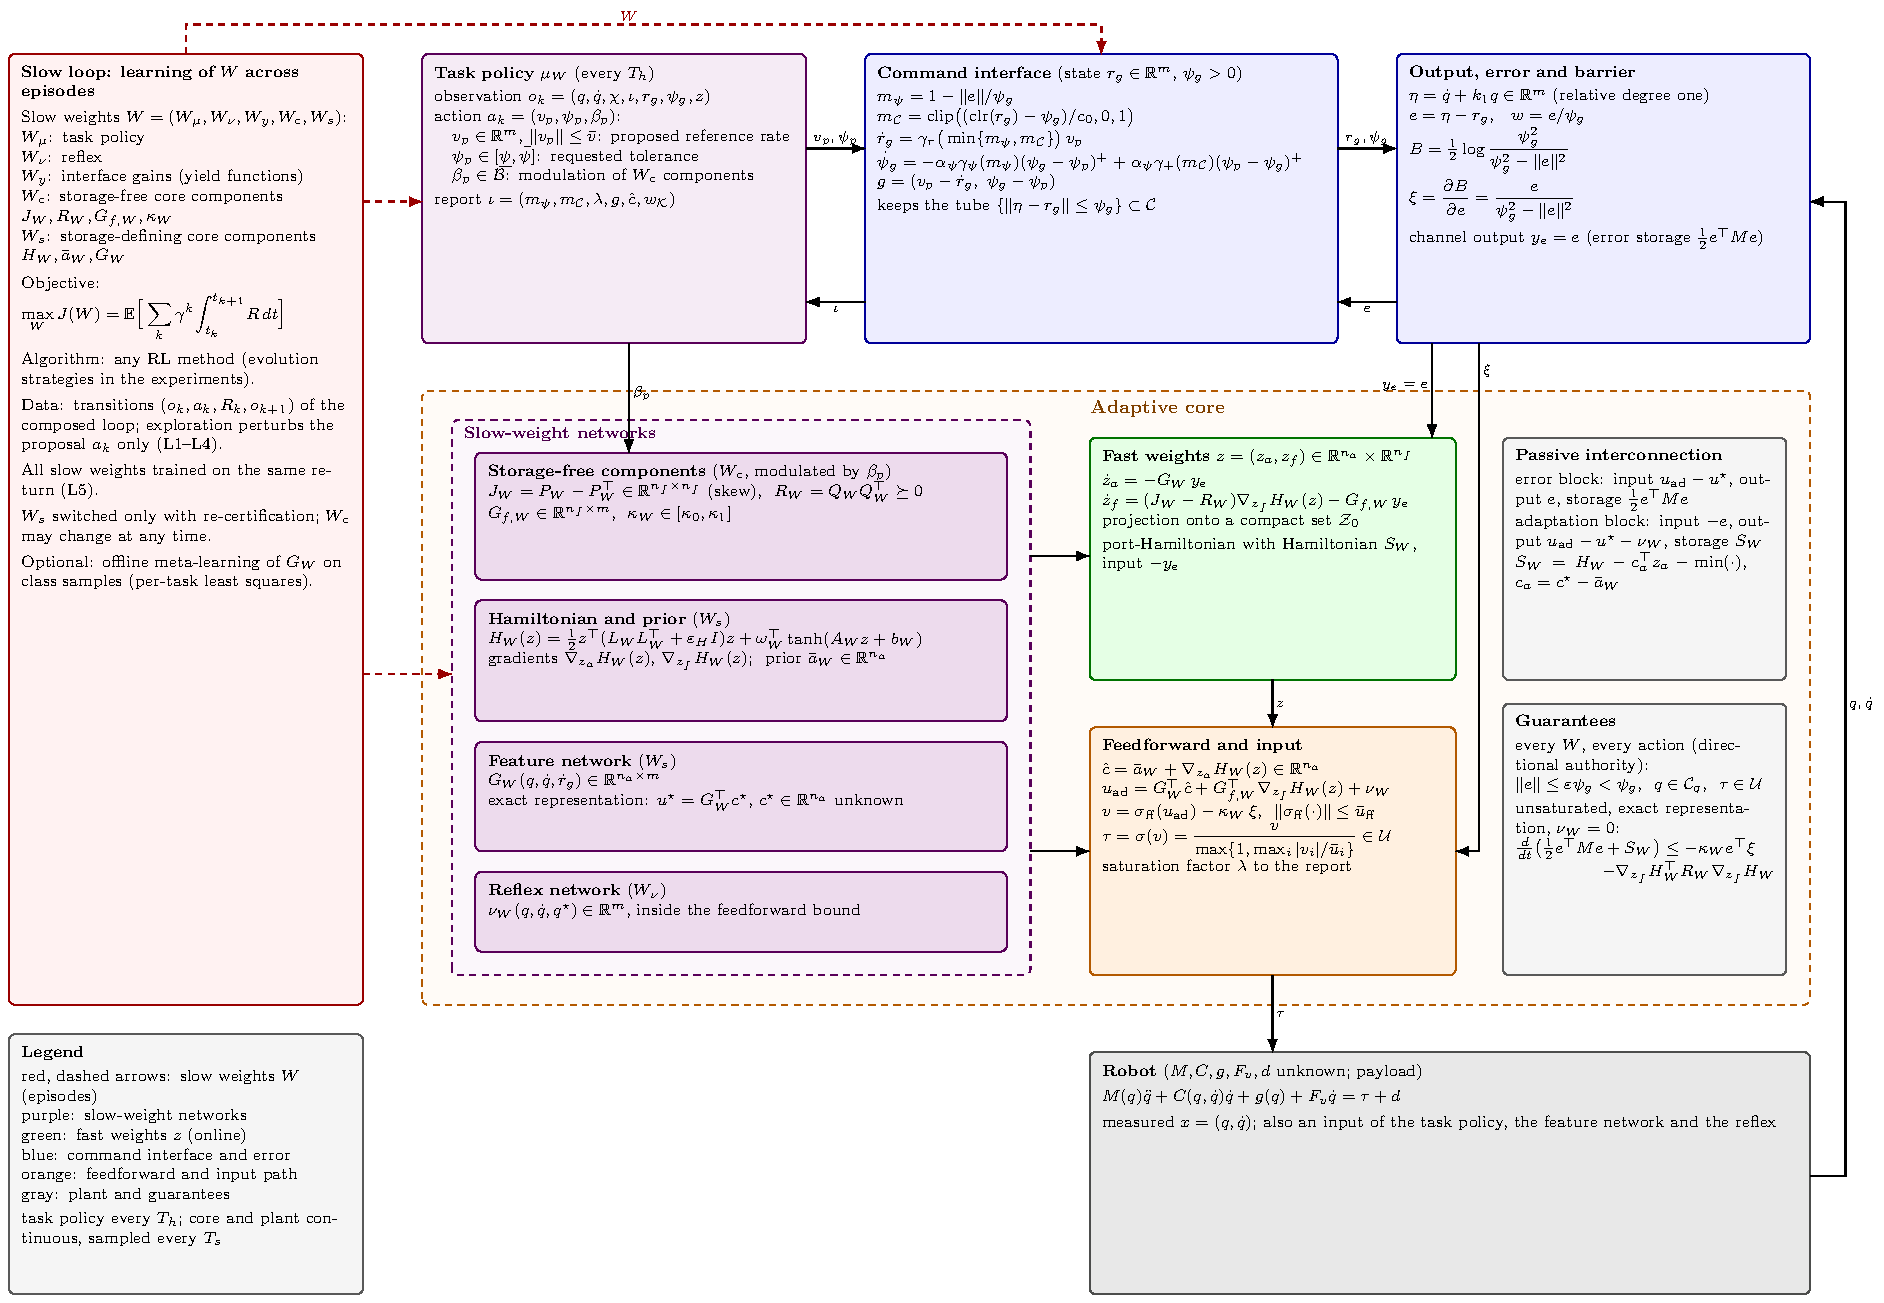
\includegraphics[width=\textheight]{architecture_v2.pdf}
\caption{Block diagram of the proposed architecture}
\label{fig:blockdiagram}
\end{sidewaysfigure}

\subsection{신호와 command interface}

\begin{definition}[Interface signals]
\label{def:signals}
\begin{itemize}
\item Proposal (action), piecewise constant with period $T_h>0$: $a:=(v_p,\psi_p,\beta_p)\in\mathcal A$ with
\begin{itemize}
\item $v_p\in\R^m$, $\|v_p\|\le\bar v$: the proposed rate of the reference;
\item $\psi_p\in[\underline\psi,\bar\psi]\subset\R_{>0}$: the requested tolerance;
\item $\beta_p\in\mathcal B\subset\R^{n_\beta}$, $\mathcal B$ compact: the modulation parameter.
\end{itemize}
\item Realized command: the interface state $(r_g,\psi_g)\in\R^m\times\R_{>0}$ of \Cref{def:interfacereal}; $r_g$ is the \textbf{\emph{reference}} and $\psi_g$ the \textbf{\emph{realized tolerance}}.
\item Tracking error and normalized error: $e:=\eta-r_g\in\R^m$ and $w:=e/\psi_g\in\R^m$.
\item Clearance: $\operatorname{clr}(r):=\inf\{\|r-y\|:\ y\in\R^m\setminus\Cset\}$ for $r\in\R^m$.
\item Margins: the error margin $m_\psi:=1-\|w\|$, the constraint margin $m_{\Cset}:=\min\{1,\max\{0,(\operatorname{clr}(r_g)-\psi_g)/c_0\}\}$ with a design constant $c_0>0$, and $m:=\min\{m_\psi,m_{\Cset}\}$.
\item \textbf{\emph{Direction-preserving}} saturation onto $\U$: $\sigma(v):=\lambda(v)\,v$ with the saturation factor $\lambda(v):=1/\max\{1,\max_i|v_i|/\bar u_i\}\in(0,1]$ for $v\in\R^m$; $\lambda=1$ iff the saturation is inactive.
\item Realization gap: $g:=(v_p-\dot r_g,\ \psi_g-\psi_p)\in\R^m\times\R$.
\end{itemize}
\end{definition}

\begin{definition}[Barrier storage and transformed error]
\label{def:barrier}
On $\mathcal E:=\{(e,\psi_g)\in\R^m\times\R_{>0}:\ \|e\|<\psi_g\}$ define
\[
B(e,\psi_g):=\tfrac12\log\frac{\psi_g^2}{\psi_g^2-\|e\|^2}=-\tfrac12\log\big(1-\|w\|^2\big),\qquad \xi:=\frac{\partial B}{\partial e}=\frac{e}{\psi_g^2-\|e\|^2}\in\R^m .
\]
\end{definition}

\begin{fact}[Properties of the barrier storage]
\label{fact:barrier}
On $\mathcal E$:
\begin{enumerate}[label=(\alph*)]
\item $B\ge0$, $\ B=0\iff e=0$, and $B\to\infty$ as $\|e\|\to\psi_g$;
\item $\xi=k\,e$ with $k:=1/(\psi_g^2-\|e\|^2)>0$, and $\|\xi\|\to\infty$ as $\|e\|\to\psi_g$;
\item $\partial B/\partial\psi_g=-\|w\|^2/\big(\psi_g(1-\|w\|^2)\big)\le0$.
\end{enumerate}
\end{fact}

\begin{proof}
(a) $0\le\|w\|^2<1$이므로 로그의 인자가 $(0,1]$에 있다.
\[
-\tfrac12\log(1-\|w\|^2)\ge0,\qquad \|w\|\to1\ \Rightarrow\ -\tfrac12\log(1-\|w\|^2)\to\infty .
\]
(b) $\|e\|^2$를 $e$로 미분하면 $2e$이다. (c) $B=\log\psi_g-\tfrac12\log(\psi_g^2-\|e\|^2)$를 미분한다.
\[
\frac{\partial B}{\partial\psi_g}=\frac1{\psi_g}-\frac{\psi_g}{\psi_g^2-\|e\|^2}=-\frac{\|e\|^2}{\psi_g(\psi_g^2-\|e\|^2)} .
\]
\end{proof}

\textbf{직관 (barrier와 CBF).} $B$는 오차가 허용 오차 경계에 다가가면 무한대가 되는 에너지이다. $B$가 유한하게 유지되면 오차는 경계에 닿지 않는다. Feedback $-\kappa\xi=-\kappa k\,e$는 gain $\kappa k$가 경계에 가까울수록 커지는 비례 제어이다. 안전 집합을 $h:=\psi_g^2-\|e\|^2\ge0$으로 쓰면 $B=-\tfrac12\log(h/\psi_g^2)$, $\xi=e/h$이고, $\psi_g$가 고정일 때 $\dot h=-2e^\top\dot e$이다. 경계 근처에서 $\kappa k$가 커지므로 $e^\top\dot e$가 강하게 음이 되어 control barrier function형 조건 $\dot h\ge-\alpha(h)$가 성립한다. CBF-QP와 달리 $\dot h$를 계산할 model이 필요 없고, 입력이 유계일 때 이것이 가능한지는 authority 조건이 보장한다.

\begin{definition}[Command interface]
\label{def:interface}
The \textbf{\emph{command interface}} is a dynamic system with state $(r_g,\psi_g)$,
\[
(\dot r_g,\dot\psi_g)=Y_W\big(a,r_g,\psi_g,m_\psi,m_{\Cset}\big),
\]
that satisfies, for every weight and every action:
\begin{itemize}
\item[\textbf{(Y1)}] (Yielding) $\|\dot r_g\|\le\gamma_r(m)\,\|v_p\|$ with $\gamma_r$ continuous, nondecreasing and $\gamma_r(0)=0$.
\item[\textbf{(Y2)}] (Yielding of the tolerance) $\dot\psi_g\ge-\bar\alpha\,\gamma_\psi(m_\psi)\,\max\{\psi_g-\psi_p,0\}$ with a constant $\bar\alpha>0$ and $\gamma_\psi$ continuous, nondecreasing, $\gamma_\psi(0)=0$; and $\dot\psi_g\le0$ whenever $m_{\Cset}=0$.
\item[\textbf{(Y3)}] (Constraint) $\{\eta:\|\eta-r_g(t)\|\le\psi_g(t)\}\subset\Cset$ $\forall t$.
\item[\textbf{(Y4)}] (Regularity) $r_g\in C^{\varrho}$ and $\psi_g\in C^1$ with bounded derivatives.
\item[\textbf{(Y5)}] (Liveness) If $m\ge m_0>0$ on an interval, then $\dot r_g=\gamma_r(m)\,v_p$ with $\gamma_r(m)\ge\gamma_r(m_0)>0$ and $\psi_g$ moves toward $\psi_p$ on that interval.
\end{itemize}
\end{definition}

\begin{definition}[Interface realization]
\label{def:interfacereal}
Let $\gamma_r,\gamma_\psi,\gamma_+:[0,1]\to[0,1]$ be Lipschitz, nondecreasing and zero at $0$ (\textbf{\emph{yield functions}}), and $\alpha_\psi>0$. The realization is
\begin{align}
\dot r_g&=\gamma_r(m)\,v_p, \label{eq:rgdot}\\
\dot\psi_g&=-\alpha_\psi\,\gamma_\psi(m_\psi)\,(\psi_g-\psi_p)^+ +\alpha_\psi\,\gamma_+(m_{\Cset})\,(\psi_p-\psi_g)^+, \label{eq:psigdot}
\end{align}
with $(\cdot)^+:=\max\{\cdot,0\}$ and initial values satisfying $\|e(0)\|<\psi_g(0)$, $\ \psi_g(0)\ge\underline\psi$, $\ \operatorname{clr}(r_g(0))\ge\psi_g(0)$.
\end{definition}

\textbf{직관 (왜 그대로 따르지 않는가).} $\dot r_g=v_p$로 두면 보장이 두 경우에 깨진다. 첫째, reference가 plant가 유계 입력으로 따라올 수 있는 것보다 빨리 움직이면 오차가 허용 오차 경계에 닿고, 그 순간 필요한 입력은 무한대이다. 둘째, reference가 제약 경계 쪽으로 계속 가면 tube가 제약 집합 밖으로 나간다. \eqref{eq:rgdot}는 두 여유 중 작은 것에 따라 진행을 늦추어 두 경우를 막는다(예: $\gamma_r(m)=\min\{1,m/m_r\}$이면 여유가 $m_r$ 이상일 때 제안을 그대로 따르고, 그 아래에서 비례해서 늦추고, 0에서 멈춘다). \eqref{eq:psigdot}에서 $\psi_g$는 요청 $\psi_p$ 쪽으로 움직이되, 줄어드는 것은 오차 여유가 있을 때만, 늘어나는 것은 제약 여유가 있을 때만 허용된다. 그래서 $\psi_p$는 요청이고 $\psi_g$는 그 요청이 실현된 상태이다. 이 실현은 (Y1)--(Y4)를 만족한다(제약 노트의 Lemma 2와 Theorem 1).

\subsection{오차 채널과 고전 적응 법칙}

\begin{definition}[Ideal input and representation]
\label{def:repr}
\begin{itemize}
\item The \textbf{\emph{ideal input}} $u^\star(t)\in\R^m$ is the input that keeps $e\equiv0$ along the realized command.
\item For a feature matrix $G(t)\in\R^{n_a\times m}$, the representation is \textbf{\emph{exact}} if $\exists\,c^\star\in\R^{n_a}$ constant with $u^\star=G^\top c^\star$ along every solution; otherwise the \textbf{\emph{residual}} is $\delta:=u^\star-G^\top c$ with $c$ minimizing $\sup\|\delta\|$ over the constraint region.
\end{itemize}
\end{definition}

\begin{assumption}[Error channel]
\label{ass:channel}
For the unsaturated input $u=u_{\mathrm{ad}}-\kappa\,\xi$ with any feedforward $u_{\mathrm{ad}}\in\R^m$ and any $\kappa>0$, there exist a $C^1$ function $V_e\ge0$ (\textbf{\emph{error storage}}), a signal $y_e\in\R^m$ (\textbf{\emph{channel output}}), a constant $\lambda_e>0$ and signals $\alpha_e\ge0$ and $\pi$, with $\pi\le0$ whenever $\dot\psi_g\ge0$, such that along every solution
\[
\dot V_e\le-\alpha_e+\lambda_e\,y_e^\top\big(u_{\mathrm{ad}}-u^\star\big)+\pi .
\]
\end{assumption}

\begin{lemma}[Two error channels]
\label{lem:channels}
\begin{enumerate}[label=(\alph*)]
\item (Relative degree one, isotropic gain) If $\varrho=1$, so that $\dot\eta=F+\Gamma u$ with the drift $F$ of (S4), and $\Gamma=\gamma I$ with a constant $\gamma>0$, then \Cref{ass:channel} holds with
\[
V_e=B,\qquad y_e=\xi,\qquad \lambda_e=\gamma,\qquad \alpha_e=\gamma\kappa\|\xi\|^2,\qquad \pi=\frac{\partial B}{\partial\psi_g}\,\dot\psi_g .
\]
\item (Mechanical systems) For the system of \Cref{rem:mech} with output $\eta=\dot q+k_1q$, $k_1>0$, \Cref{ass:channel} holds with
\[
V_e=\tfrac12\,e^\top M(q)\,e,\qquad y_e=e,\qquad \lambda_e=1,\qquad \alpha_e=\kappa\,e^\top\xi=\frac{\kappa\|e\|^2}{\psi_g^2-\|e\|^2},\qquad \pi=0 .
\]
\end{enumerate}
\end{lemma}

\begin{proof}
(a) 이상 입력은 $u^\star=\gamma^{-1}(\dot r_g-F)$이므로 오차 동역학은 다음과 같다.
\[
\dot e=\dot\eta-\dot r_g=\gamma\,(u-u^\star)=\gamma\,(u_{\mathrm{ad}}-u^\star)-\gamma\kappa\,\xi .
\]
$B$를 미분한다.
\[
\dot B=\xi^\top\dot e+\frac{\partial B}{\partial\psi_g}\dot\psi_g=\gamma\,\xi^\top(u_{\mathrm{ad}}-u^\star)-\gamma\kappa\|\xi\|^2+\pi .
\]
\Cref{fact:barrier}(c)에 의해 $\dot\psi_g\ge0$이면 $\pi\le0$이다. (b) 제약 노트의 Proposition 3 증명 Step 1에서 $\dot M-2C$의 skew 성질로 다음을 얻는다.
\[
\frac{d}{dt}\tfrac12\,e^\top Me=e^\top(u-u^\star)=e^\top(u_{\mathrm{ad}}-u^\star)-\kappa\,e^\top\xi .
\]
\end{proof}

\begin{lemma}[Classical adaptive law as a passive interconnection]
\label{lem:classical}
Let \Cref{ass:channel} hold, let the representation be exact with a feature matrix $G(t)\in\R^{n_a\times m}$ and $c^\star\in\R^{n_a}$, and let $\Gamma_a\in\R^{n_a\times n_a}$, $\Gamma_a=\Gamma_a^\top\succ0$. With
\[
u_{\mathrm{ad}}=G^\top\hat c,\qquad \dot{\hat c}=-\Gamma_a\,G\,y_e,\qquad \tilde c:=\hat c-c^\star,\qquad V:=V_e+\tfrac{\lambda_e}{2}\,\tilde c^\top\Gamma_a^{-1}\tilde c,
\]
every solution satisfies
\[
\dot V\le-\alpha_e+\pi .
\]
\end{lemma}

\begin{proof}
Mismatch는 $u_{\mathrm{ad}}-u^\star=G^\top\tilde c$이다. 두 storage를 따로 미분한다.
\[
\dot V_e\le-\alpha_e+\lambda_e\,y_e^\top G^\top\tilde c+\pi .
\]
\[
\frac{\lambda_e}{2}\frac{d}{dt}\big(\tilde c^\top\Gamma_a^{-1}\tilde c\big)=\lambda_e\,\tilde c^\top\Gamma_a^{-1}\dot{\hat c}=-\lambda_e\,\tilde c^\top G\,y_e .
\]
두 식을 더하면 교차항이 사라진다.
\end{proof}

\textbf{해석 (두 passive block).} 적응 block은 상태 $\tilde c$, 입력 $-y_e$, 출력 $G^\top\tilde c$를 가진 port-Hamiltonian system이다. Hamiltonian은 $\tfrac12\tilde c^\top\Gamma_a^{-1}\tilde c$, 구조는 $\mathcal J=\mathcal R=0$, port matrix는 $\Gamma_aG$이다. 오차 block은 그 출력을 입력으로 받는 passive block이고, \Cref{lem:classical}의 교차항 상쇄는 \Cref{lem:interconnect}이다. $V$는 두 block의 storage의 합이다.

\subsection{Adaptive core}

\textbf{직관 (적분기를 port-Hamiltonian system으로).} \Cref{lem:classical}의 증명은 적응 block이 passive하다는 것만 쓴다. 따라서 적분기를 다른 port-Hamiltonian system으로 바꾸어도 교차항은 같은 방식으로 상쇄되고, 그 $H$, $\mathcal J$, $\mathcal R$, port matrix를 network로 두면 모든 weight에서 같은 결론이 나온다(\Cref{thm:balance}). 상태는 둘로 나눈다. $z_a$는 감쇠 없이 적분하는 부분으로, 정확한 이상 입력에 도달하는 적분 동작을 맡는다. $z_f$는 오차 신호를 가공하는 내부 기억으로, $R_W$로 잊기와 filtering을, $J_W$로 momentum이나 진동 모드(\Cref{rem:phex})를 표현한다. $H_W$가 2차가 아니면 적응 속도가 상태에 따라 달라진다.

\begin{definition}[Hamiltonian class]
\label{def:hclass}
Let $n_z:=n_a+n_f$ and fix $\varepsilon_H>0$. For $z=(z_a,z_f)\in\R^{n_a}\times\R^{n_f}$,
\[
H_W(z):=\tfrac12\,z^\top\big(L_WL_W^\top+\varepsilon_HI_{n_z}\big)z+\omega_W^\top\tanh\big(A_Wz+b_W\big),
\]
with weights $L_W\in\R^{n_z\times n_z}$, $A_W\in\R^{n_h\times n_z}$ and $b_W,\omega_W\in\R^{n_h}$, $\tanh$ applied componentwise.
\end{definition}

\begin{fact}[Properties of the Hamiltonian class]
\label{fact:hclass}
For every weight:
\begin{enumerate}[label=(\alph*)]
\item $H_W\in C^\infty$ and $\nabla H_W$ is globally Lipschitz;
\item $H_W(z)\ge\tfrac{\varepsilon_H}{2}\|z\|^2-\|\omega_W\|_1$ $\ \forall z$;
\item $\forall\,c\in\R^{n_a}$, the function $z\mapsto H_W(z)-c^\top z_a$ attains its minimum on $\R^{n_z}$.
\end{enumerate}
\end{fact}

\begin{proof}
(a) Gradient와 Hessian을 쓴다($s:=\tanh(A_Wz+b_W)$, $\odot$는 성분별 곱).
\[
\nabla H_W=(L_WL_W^\top+\varepsilon_HI)z+A_W^\top\big(\omega_W\odot(1-s\odot s)\big).
\]
\[
\nabla^2H_W=L_WL_W^\top+\varepsilon_HI-2A_W^\top\operatorname{diag}\big(\omega_W\odot s\odot(1-s\odot s)\big)A_W .
\]
$|s_i(1-s_i^2)|\le1$이므로 Hessian이 유계이다. (b) $|\tanh|\le1$에서 다음이 나온다.
\[
\big|\omega_W^\top\tanh(A_Wz+b_W)\big|\le\|\omega_W\|_1 .
\]
(c) (b)를 쓴다.
\[
H_W(z)-c^\top z_a\ge\tfrac{\varepsilon_H}{2}\|z\|^2-\|c\|\,\|z\|-\|\omega_W\|_1\ \longrightarrow\ \infty\quad(\|z\|\to\infty),
\]
연속 함수가 coercive하므로 최솟값에 도달한다.
\end{proof}

\begin{definition}[Adaptive core]
\label{def:core}
Let $y_e\in\R^m$ be the channel output of \Cref{ass:channel}. The \textbf{\emph{adaptive core}} has fast weights $z=(z_a,z_f)\in\R^{n_a}\times\R^{n_f}$ and the components
\begin{itemize}
\item feature matrix $G_W(t)\in\R^{n_a\times m}$, a network of the measured signals and the realized command;
\item internal port matrix $G_{f,W}(t)\in\R^{n_f\times m}$;
\item interconnection $J_W\in\R^{n_f\times n_f}$ with $J_W=-J_W^\top$, and dissipation $R_W\in\R^{n_f\times n_f}$ with $R_W=R_W^\top\succeq0$;
\item Hamiltonian $H_W$ of \Cref{def:hclass} and prior $\bar a_W\in\R^{n_a}$;
\item reflex $\nu_W(t)\in\R^m$, a network of the measured signals;
\item barrier gain $\kappa_W\in[\kappa_0,\kappa_1]$ with fixed $0<\kappa_0\le\kappa_1$, and feedforward bound $\bar u_{\mathrm{ff}}\ge0$.
\end{itemize}
Its dynamics and output are
\begin{align}
\dot z_a&=-G_W\,y_e, \label{eq:za}\\
\dot z_f&=(J_W-R_W)\,\nabla_{z_f}H_W(z)-G_{f,W}\,y_e, \label{eq:zf}\\
\hat c&:=\bar a_W+\nabla_{z_a}H_W(z)\in\R^{n_a}, \label{eq:chat}\\
u_{\mathrm{ad}}&:=G_W^\top\hat c+G_{f,W}^\top\nabla_{z_f}H_W(z)+\nu_W\in\R^m, \label{eq:uad}\\
u&=\sigma\big(\sigma_{\mathrm{ff}}(u_{\mathrm{ad}})-\kappa_W\,\xi\big)\in\U, \label{eq:u}
\end{align}
where $\sigma_{\mathrm{ff}}(v):=v\,\min\{1,\bar u_{\mathrm{ff}}/\|v\|\}$, and a projection onto a compact set $\mathcal Z_0\subset\R^{n_z}$ is applied to \eqref{eq:za}--\eqref{eq:zf}. The modulation $\beta_p$ of \Cref{def:signals} selects $(J_W,R_W,\kappa_W,G_{f,W})$ within these sets at each tick, and the \textbf{\emph{report}} is $\iota:=(m_\psi,m_{\Cset},\lambda,g,\hat c,w_{\Kset})$, where $w_{\Kset}\ge0$ is the diameter of the certified parameter set $\Kset_t\subset\R^{n_a}$.
\end{definition}

\begin{definition}[Adaptation storage]
\label{def:storage}
If the representation is exact with $c^\star\in\R^{n_a}$ for $G=G_W$, let $c_a:=c^\star-\bar a_W$ and
\[
S_W(z):=H_W(z)-c_a^\top z_a-\min_{z'\in\R^{n_z}}\big\{H_W(z')-c_a^\top z'_a\big\}\ \ge0 .
\]
\end{definition}

\begin{lemma}[The fast-weight dynamics are port-Hamiltonian]
\label{lem:corepH}
Let the representation be exact with $c^\star$. Without projection, \eqref{eq:za}--\eqref{eq:zf} is the port-Hamiltonian system with Hamiltonian $S_W$, input $-y_e$ and
\[
\mathcal J=\begin{pmatrix}0&0\\0&J_W\end{pmatrix},\qquad \mathcal R=\begin{pmatrix}0&0\\0&R_W\end{pmatrix},\qquad \mathcal G=\begin{pmatrix}G_W\\ G_{f,W}\end{pmatrix}\in\R^{n_z\times m},
\]
whose output is the feedforward mismatch without the reflex,
\[
y_c:=\mathcal G^\top\nabla S_W=u_{\mathrm{ad}}-u^\star-\nu_W .
\]
Consequently, for every weight and every modulation,
\[
\dot S_W=-\nabla_{z_f}H_W^\top R_W\,\nabla_{z_f}H_W-y_e^\top y_c .
\]
\end{lemma}

\begin{proof}
$S_W$의 gradient를 \eqref{eq:chat}로 쓴다.
\[
\nabla_{z_a}S_W=\nabla_{z_a}H_W-c_a=\hat c-c^\star,\qquad \nabla_{z_f}S_W=\nabla_{z_f}H_W .
\]
\Cref{def:ph}의 우변에 넣으면 행별로 \eqref{eq:za}와 \eqref{eq:zf}가 된다.
\[
\big((\mathcal J-\mathcal R)\nabla S_W-\mathcal G\,y_e\big)_a=-G_Wy_e,\qquad \big((\mathcal J-\mathcal R)\nabla S_W-\mathcal G\,y_e\big)_f=(J_W-R_W)\nabla_{z_f}H_W-G_{f,W}\,y_e .
\]
출력을 \eqref{eq:uad}와 $u^\star=G_W^\top c^\star$로 쓴다.
\[
\mathcal G^\top\nabla S_W=G_W^\top(\hat c-c^\star)+G_{f,W}^\top\nabla_{z_f}H_W=u_{\mathrm{ad}}-\nu_W-u^\star .
\]
마지막 식은 \Cref{lem:phpassive}에 입력 $-y_e$를 넣은 것이다.
\end{proof}

\begin{theorem}[Storage balance of the core]
\label{thm:balance}
Let \Cref{ass:channel} hold, let the representation be exact with $c^\star$, and let $\nu_W\equiv0$. On every interval on which $\lambda(\cdot)=1$, $\|u_{\mathrm{ad}}\|\le\bar u_{\mathrm{ff}}$ and the projection is inactive, the function
\[
V:=V_e+\lambda_e\,S_W
\]
satisfies, for every weight and every modulation $\beta_p$,
\begin{enumerate}[label=(\alph*)]
\item $\dot V\le-\alpha_e-\lambda_e\,\nabla_{z_f}H_W^\top R_W\nabla_{z_f}H_W+\pi$;
\item if in addition $\dot\psi_g\ge0$ on the interval $[t_0,t_1)$, then $V$ is nonincreasing and $\int_{t_0}^{t_1}\alpha_e\,dt\le V(t_0)$.
\end{enumerate}
The scope is the unsaturated, projection-free regime with exact representation; the constraint guarantees of \Cref{sec:requirements} do not depend on these conditions.
\end{theorem}

\begin{proof}
조건 아래에서 $u=u_{\mathrm{ad}}-\kappa_W\xi$이므로 \Cref{ass:channel}이 적용되고, $\nu_W=0$이므로 \Cref{lem:corepH}의 출력은 mismatch 전체이다.
\[
\dot V_e\le-\alpha_e+\lambda_e\,y_e^\top y_c+\pi,\qquad \lambda_e\dot S_W=-\lambda_e\nabla_{z_f}H_W^\top R_W\nabla_{z_f}H_W-\lambda_e\,y_e^\top y_c .
\]
두 식을 더하면 (a)이다. (b)는 $\pi\le0$와 $V\ge0$에서 (a)를 적분한 것이다.
\end{proof}

\begin{remark}[Special cases and the experiments]
\label{rem:coreinst}
$n_f=0$, $L_W=0$, $\omega_W=0$이면 $H_W=\tfrac{\varepsilon_H}{2}\|z_a\|^2$이고 \eqref{eq:chat}과 \eqref{eq:za}는 고전 법칙이 된다($\Gamma_a=\varepsilon_HI$).
\[
\hat c=\bar a_W+\varepsilon_Hz_a,\qquad \dot{\hat c}=-\varepsilon_H\,G_W\,y_e .
\]
학습 비교 실험의 core는 이 경우이다. Feature 벡터 $\Phi(t)\in\R^{N}$와 행렬 $\hat W\in\R^{N\times m}$에 대해 $\hat c=\operatorname{vec}(\hat W)$, $G_W=I_m\otimes\Phi\in\R^{Nm\times m}$로 두면 $G_W^\top\hat c=\hat W^\top\Phi$이다. 이때 $\varepsilon_H=g_a$, $y_e=e$(\Cref{lem:channels}(b))이며, $\bar a_W$는 학습된 초기값이다.
\end{remark}

\begin{remark}[Storage-free components and the reflex]
\label{rem:storagefree}
$S_W$는 $H_W$, $\bar a_W$, $G_W$에만 의존한다($G_W$는 $c^\star$를 정한다). $J_W$, $R_W$, $G_{f,W}$, $\kappa_W$는 $S_W$에 나타나지 않으므로 \Cref{thm:balance}는 이들이 시간에 따라 임의로 바뀌어도 성립하며, $\beta_p$는 이 성분들만 조절한다. Reflex $\nu_W$는 $\dot V$에 공급항 $\lambda_e y_e^\top\nu_W$를 더하므로 \Cref{thm:balance}의 가정에서 제외되지만, 유계인 feedforward의 일부이므로 제약 보장에는 영향이 없다. 비등방 input gain에서 \Cref{lem:channels}(a)가 성립하지 않는 것은 $\dot B=\xi^\top\Gamma(u-u^\star)$의 출력 $\Gamma^\top\xi$를 모르기 때문이며, 기계 system에서는 storage를 $M$으로 가중해 출력이 $e$가 된다.
\end{remark}

\begin{definition}[Task policy and weights]
\label{def:weights}
\begin{itemize}
\item The \textbf{\emph{task policy}} $\mu_W:(x,\chi,\iota,r_g,\psi_g,z)\mapsto a$ is an arbitrary network, evaluated every $T_h$.
\item Slow weights: $W:=(W_\mu,W_\nu,W_y,W_c,W_s)$ for the task policy, the reflex, the interface gains, the storage-free core components $(J_W,R_W,\kappa_W,G_{f,W})$ and the storage-defining components $W_s:=(H_W,\bar a_W,G_W)$.
\item Free weights: $W_{\mathrm{free}}:=(W_\mu,W_\nu,W_y,W_c)$.
\item Fast weights: $z\in\R^{n_z}$, updated by \eqref{eq:za}--\eqref{eq:zf} every $T_s$, with $T_h=NT_s$.
\end{itemize}
\end{definition}

\textbf{해석 (비선형성의 위치).} Fast weight $z_a$가 feature $G_W$에 선형으로 들어가는 것은 \Cref{lem:corepH}에서 출력이 mismatch와 같아지는 조건이다. 비선형성은 $H_W$의 geometry, 학습되는 feature, 내부 기억 $z_f$, reflex, interface의 gain, task policy에 있으며, reflex와 task policy에는 구조 제한이 없다. $\kappa_W$가 scalar이고 saturation이 방향을 보존하는 것은 input gain이 대각이 아닐 때 feedback이 오차를 줄이는 방향을 유지하기 위한 조건이다.


\section{학습 문제}
\label{sec:mdp}

\begin{definition}[Decision process]
\label{def:mdp}
At decision times $t_k:=kT_h$ let $s_k:=(x,z,r_g,\psi_g,\Kset_{t_k},\chi)$ and let $P_\theta$ be the transition induced by \eqref{eq:plant}, \Cref{def:core,def:interface} over $[t_k,t_{k+1})$ with $a_k$ held constant. The learning problem is
\[
\max_W\ J(W):=\mathbb E_{\chi,\theta,s_0}\Big[\sum_{k\ge0}\gamma^k\!\int_{t_k}^{t_{k+1}}\!R(x,u,\chi)\,dt\Big],\qquad a_k=\mu_W(o_k),\quad o_k:=(x,\chi,\iota,r_g,\psi_g,z)(t_k),
\]
where $\theta$ is not observed. Training uses any RL algorithm; no constraint term is added to $R$.
\end{definition}

\begin{definition}[Learning-time coupling]
\label{def:learn}
The learning process satisfies, with $R_k:=\int_{t_k}^{t_{k+1}}R\,dt$:
\begin{itemize}
\item[\textbf{(L1)}] (Composed loop, exploration through the command) Every transition used for learning is generated by the closed loop of \eqref{eq:plant} and \Cref{def:core,def:interface}; the only signal chosen by the learner is the proposal $a_k\in\mathcal A$, and exploration perturbs $a_k$, not $u$.
\item[\textbf{(L2)}] (No hidden state of the lower parts) $o_k$ determines $(z,r_g,\psi_g)$ at $t_k$, so that the only unobserved quantities of the decision process are $\theta$ and $d$.
\item[\textbf{(L3)}] (Reports are measurements) $m_\psi$, $m_{\Cset}$, $\lambda$ and $g$ are functions of signals realized up to $t_k$ and contain no prediction; they keep their meaning $\forall W$ and while $W$ varies.
\item[\textbf{(L4)}] (Attribution) A transition is recorded as $(o_k,a_k,R_k,o_{k+1})$ with the proposal $a_k$ as the action; $o_{k+1}$ contains the realization gap accumulated on $[t_k,t_{k+1})$; and the map $Y_W$ from the proposal to the command derivatives is known to the learner in closed form.
\item[\textbf{(L5)}] (Joint training) All slow weights, those of the task policy and those of the core and the interface, are trained on the same return $J(W)$ through the composed loop.
\end{itemize}
\end{definition}

\textbf{해석 (RL이 보는 것).} $\theta$는 관측되지 않으므로 이 문제는 부분 관측 문제이고, core의 보고 $\iota$가 $\theta$에 대한 통계량 역할을 한다. Task policy는 허용 오차와 진행 속도를 action으로 가지므로, 정밀도가 필요한 때와 불확실성을 줄이기 위해 움직일 때를 스스로 정한다.

\textbf{해석 (학습 중에 오가는 지식).} 아래층이 지금 무엇을 할 수 있는지는 사전에 계산해 주지 않는다. Task policy는 제안이 얼마나 늦춰지고 요청한 허용 오차가 얼마나 실현되는지를 보고에서 관측하고, 그 관계를 return을 통해 학습한다. 반대 방향으로는 core와 interface의 slow weight가 같은 return으로 학습되므로, 아래층은 위층이 실제로 내는 명령의 분포에 맞춰진다. (L2)에 의해 fast weight의 적응은 숨은 환경 변화가 아니라 관측되는 상태의 변화이다. (L1)은 탐색이 command를 통해서만 일어나게 한다.

\section{보장 요구 사항}
\label{sec:requirements}
\label{sec:req}

\begin{assumption}[Admissibility]
\label{ass:adm}
\begin{itemize}
\item[\textbf{(C1)}] (Initial condition) $\|e(0)\|<\psi_g(0)$ and the initial tube lies in $\Cset$.
\item[\textbf{(C2)}] (Input authority) A constant $\rho_0>0$, computable from the class data, bounds from below the rate at which the saturated input along the restoring direction reduces the error coordinate of relative degree one, $\forall\theta\in\Theta$ on the constraint region. For $\varrho=1$ a sufficient condition is $\gamma_0\min_i\bar u_i-\bar F>0$ with $\bar F$ the envelope of (S4); for mechanical systems the condition is evaluated direction by direction.
\item[\textbf{(C3)}] (Residual) $\sup\|\delta\|\le\bar\delta$ on the constraint region, with $\bar\delta$ finite.
\item[\textbf{(C4)}] (Exogenous signals) $\chi$ and $d$ are bounded.
\end{itemize}
\end{assumption}

\begin{definition}[Guarantee requirements]
\label{def:req}
The following are required $\forall\,W$, $\forall$ action sequence $\{a_k\}\subset\mathcal A$, $\forall\,\theta\in\Theta$, $\forall\,\chi$ and every initial condition satisfying (C1).

\emph{Tier 1 (by construction).}
\begin{itemize}
\item[\textbf{(Q1)}] (Tolerance) $\|e(t)\|<\psi_g(t)$ $\forall t\ge0$.
\item[\textbf{(Q2)}] (State constraint) $\eta(t)\in\Cset$ $\forall t\ge0$.
\item[\textbf{(Q3)}] (Input constraint) $u(t)\in\U$ $\forall t\ge0$.
\item[\textbf{(Q4)}] (Well-posedness) The closed loop has a unique solution on $[0,\infty)$, the interface is defined $\forall t$, and $z$, $r_g$, $\psi_g$ are bounded by constants computable a priori from the class data.
\item[\textbf{(Q5)}] (Learning invariance) (Q1)--(Q4) hold under arbitrary measurable time variation of all weights and for every exploration signal in $\mathcal A$. The properties that rest on the storage, (Q7), (Q8) and $\Kset_t$, hold under arbitrary variation of $W_{\mathrm{free}}$ and under switching of $W_s$ that is re-certified with $\Kset_t$.
\item[\textbf{(Q6)}] (Knowledge and certificates) The policy uses only the class data of \Cref{def:plant,def:constraints}; every certificate is a priori, non-circular, and closed-form or computable offline without simulation.
\item[\textbf{(L1)--(L5)}] (Learning-time coupling) The conditions of \Cref{def:learn}, imposed on the learning process by construction.
\end{itemize}

\emph{Tier 2 (properties to prove).}
\begin{itemize}
\item[\textbf{(Q7)}] (Intent realization) If the proposal converges to a constant target $\bar r$ with tube of radius $\psi_p$ inside $\Cset$, then $r_g\to\bar r$ and $\psi_g\to\psi_p$; if in addition $\delta\equiv0$, then $e(t)\to0$.
\item[\textbf{(Q8)}] (Capability) If $\delta\equiv0$, then along a constant realizable proposal the saturation becomes inactive ($\lambda\to1$), the realization gap vanishes ($g\to0$), and $\int_0^\infty\|\xi\|^2dt<\infty$.
\item[\textbf{(Q9)}] (Expressivity) $\mu_W$ and $\nu_W$ are unrestricted networks, and the adaptive core is dense in the set of operators of the form \eqref{eq:za}--\eqref{eq:u}; hence every policy of this architecture with continuous components is approximated on compact sets.
\item[\textbf{(Q10)}] (Sampled data) (Q1)--(Q4) hold for the implementation with periods $(T_s,T_h)$ under an explicit bound on $T_s$.
\item[\textbf{(Q11)}] (Complexity) No online optimization is used; the computation per tick is of the order of one evaluation of the networks, and the order of the fast loop is $n_a+n_f$.
\end{itemize}

\emph{Tier 3 (empirical objectives).}
\begin{itemize}
\item[\textbf{(Q12)}] (Performance) The return is not lower than that of the baselines of \Cref{sec:eval} at zero constraint violations, during and after training.
\item[\textbf{(Q13)}] (Necessity of the coupling) Removing any one of the tolerance action, the yielding (Y1)--(Y2), the reports and the fast weights in the observation (L2)--(L4), or the joint training (L5) either breaks a Tier~1 property or lowers the return.
\end{itemize}
\end{definition}

\begin{definition}[Contract between the parts]
\label{def:contract}
\begin{itemize}
\item Core contract. \emph{Assumes}: (C1)--(C4), the yielding (Y1)--(Y2) and (Y4). \emph{Guarantees}: (Q1) with an a priori bound on $\|e\|/\psi_g$, (Q3), and the reports $m_\psi$, $\lambda$.
\item Interface contract. \emph{Assumes}: nothing about the plant or the core. \emph{Guarantees}: (Y1)--(Y4) for every action and every signal $m_\psi\in[0,1]$; (Y5) is a property to prove.
\item Task policy. No obligation.
\item Composition. The reports at time $t$ depend on signals on $[0,t]$ only and the command derivatives at $t$ depend on the reports at $t$ only; the two contracts then imply (Q1)--(Q4).
\end{itemize}
\end{definition}

\textbf{해석 (보장이 한쪽에만 있지 않다).} Input 제약 때문에 core의 보장은 interface가 여유에 따라 진행과 수축을 늦출 때만 성립하고, state 제약은 core가 허용 오차를 지킬 때만 성립한다. 따라서 Tier 1은 두 계약의 합성으로만 얻어진다. Task policy에는 의무가 없으므로 RL은 제약 없는 문제를 풀고, 무엇이 실현되는지는 보고에서 배운다.

\section{핵심 아이디어와 그 역할}
\label{sec:ideas}

\begin{table}[H]
\centering\footnotesize\setlength{\tabcolsep}{4pt}
\caption{Adaptive-control principles, mechanisms and the requirements they serve}
\label{tab:ideas}
\begin{tabular}{p{3.6cm}p{6.2cm}p{4.6cm}}
\toprule
적응 제어의 원리 & 이 구조의 기제 & 대응하는 요구 \\
\midrule
High-gain 적응 (funnel 제어) & 명령된 허용 오차에 대한 barrier storage $B(e,\psi_g)$와 변환된 오차 $\xi$ & (Q1): 사전 parameter 집합 없이 class 조건만으로 \\
Hyperstability, 미지 값을 storage 기준점에만 두는 것 & Fast weight의 port-Hamiltonian 구조, storage는 $W_s$에만 의존 & (Q5), (Q9), (Q7)의 정확한 수렴 \\
오차를 듣는 reference model & 여유에 따라 진행과 수축을 늦추는 command interface & (Q1), (Q2), (Q4) \\
적응의 부산물로서의 식별 & Storage 항등식에서 얻는 인증 집합 $\Kset_t$ & (Q8), (Q5)의 재인증 \\
Certainty equivalence & Task policy는 보고를, core는 명령을 참으로 둔다 & 역할 분배, (Q13) \\
Dual effect & 허용 오차와 진행 속도가 action & (Q8), (Q12) \\
\bottomrule
\end{tabular}
\end{table}

\begin{table}[H]
\centering\footnotesize\setlength{\tabcolsep}{4pt}
\caption{Limiting assumption removed by each component}
\label{tab:synergy}
\begin{tabular}{p{4.0cm}p{10.4cm}}
\toprule
요소 & 제거하는 제한 \\
\midrule
Barrier storage & Storage 상한으로 계산한 tube가 사전 parameter 집합에 의존하고 느슨하다는 제한 \\
Command interface의 양보 & Input 제약 아래에서 허용 오차의 경계를 넓히는 방법은 넓어지는 양에 상한이 없다는 제한 \\
방향 보존 saturation & 대각이 아닌 input gain에서 성분별 saturation이 오차를 키울 수 있다는 제한 \\
Fast weight의 적응 & Funnel 제어가 경계 근처에서 계속 큰 feedback을 쓴다는 제한 \\
측정된 보고와 그 위의 학습 & 실현 가능한 속도와 정밀도를 최악 경우로 미리 계산해야 한다는 제한 \\
인증 집합 $\Kset_t$ & Storage를 정하는 weight를 배치 중 바꿀 수 없다는 제한 \\
RL & 허용 오차, 진행 속도, 탐색의 trade-off를 사람이 정해야 한다는 제한 \\
\bottomrule
\end{tabular}
\end{table}

\section{현재 상태}
\label{sec:status}

\begin{table}[H]
\centering\footnotesize\setlength{\tabcolsep}{4pt}
\caption{Status of each element}
\label{tab:status}
\begin{tabular}{p{4.6cm}p{2.3cm}p{7.5cm}}
\toprule
항목 & 상태 & 근거 \\
\midrule
Storage가 $W_s$에만 의존, free weight의 임의 변화 허용 & 증명 (exact representation) & 이전 노트의 corollary. 수치 확인은 변화 진폭 0.3까지 \\
Core의 universal approximation & 증명 (이전 class) & Barrier 형태에 대해서는 다시 확인 필요 \\
Barrier core의 (Q1), 입력 제약 없음 & 유도 ($\varrho=1$, scalar) & 64개 경우에서 이탈 0, barrier 없는 같은 법칙은 52개 이탈. Feedback effort 중앙값 0.131에서 0.075로 감소 \\
Storage 항등식의 인증 집합 & 유도, scalar 수치 & 참값 항상 포함. 폭이 사전 대비 3\% 이하(완만한 reference), 0.2\% 이하(probing) \\
(Q1)--(Q5), $\varrho=1$: core와 interface의 합성 & 증명 (충분조건) & 별도 노트의 정리. 부등식의 점 평가 $1.2\times10^7$개에서 위반 0, simulation 64개 경우에서 이탈 0, 양보를 빼면 64개 모두 이탈 \\
보고 신호(여유, saturation factor, 실현 차이) & 정의로 해결 & 측정값이어서 유효성의 증명이 필요 없음. 이전의 $\hat\psi_{\min}$을 대체 \\
기계 system에서의 authority & 수치 확인 & 가장 약한 방향으로 잰 조건은 7-DOF 표본 전부에서 성립하지 않음. 방향별 조건은 전부에서 성립(drift 배율 최소 1.09). 사전 여유는 작음 \\
진행 보장 (Y5), (Q7) & 미해결 & $\partial\Cset$ 근처에서 멀어지는 방향의 진행도 늦춰짐 \\
양보의 소멸과 storage의 감소, isotropic gain과 정확한 표현 ($\varrho=1$) & 증명 (조건부) & 별도 노트의 proposition. Saturation이 작동하지 않는 구간에서 storage 비증가와 $e\to0$. 같은 gain에서 오차 여유의 yield factor는 feedback만 쓸 때와 적응을 쓸 때 0.944 대 1.000 \\
관성 행렬을 모르는 기계 system에서의 storage 감소 & 증명 (정확한 표현) & 오차로 구동되는 fast weight와 운동 에너지 형태의 storage. 2-link arm에서 오차 여유의 yield factor는 feedback만 쓸 때와 적응을 쓸 때 0.128 대 1.000 \\
정확히 표현되지 않는 경우와 지속되는 saturation에서의 수렴, (Q8) & 미해결 & 지속되는 saturation에서 fast weight의 storage가 커지는 것을 수치로 확인 \\
Fast weight의 구동 신호 & 해결 & \Cref{def:core}가 오차 채널의 출력 $y_e$로 구동되도록 정의함: barrier 채널에서는 $\xi$, 기계 system에서는 $e$ (\Cref{lem:channels}) \\
기계 system의 제약 보장 & 증명 (볼록한 위치 제약) & Output $\dot q+k_1q$로 상대 차수 1의 정리가 적용됨. 속도 제약의 직접 지정과 볼록하지 않은 제약은 미해결 \\
학습 중의 결합 (L1)--(L5) & 시험함 & 같은 예산의 학습에서 보고는 return을 높이지 않음 \\
학습 비교 (Q12), (Q13), 2-link arm & 부정 & 입력 policy와 funnel filter의 관절 오차 0.289--0.307 rad, 제안한 구조 0.517--0.597 rad. 양쪽 모두 관절 제약 위반 0 \\
정상 상태 정확도, 사전 등록 & 부정 & 예측 기각(제안한 구조 0.422--0.448 rad, 입력 policy 0.119--0.175 rad). 규칙에 따라 이 설계는 중단 \\
원인 확인, 사전 등록 & 부정 & 네 진단 모두 기각. 네 수리를 합쳐도 관절 오차 0.455--0.471 rad로 기준 0.429 rad 미달. 다음 설계에서 허용 오차 계층을 버림 \\
Class 상한만으로의 $\Kset_t$ & 미해결 & 관성 행렬을 범위로만 알 때 정보량 미확인 \\
Sampled-data (Q10) & 미해결 & Funnel 제어의 sampled-data 결과가 문헌에 있음 \\
이 구조에서의 RL 학습 & 시작 전 & \\
\bottomrule
\end{tabular}
\end{table}

\section{평가 사양}
\label{sec:eval}

\textbf{대상.} Scalar plant($\varrho=1$), 2-link arm과 7-DOF arm($\varrho=2$, 관절 한계와 torque 한계, regressor 밖 torque 포함). Policy에는 instance model을 넣지 않는다.

\textbf{비교 대상.}
\begin{itemize}
\item Reference를 내는 RL과 고정된 강건 tube의 적응 추종을 쌓은 구조.
\item 허용 오차가 고정된 funnel 안전장치와 RL(허용 오차 action, 양보, 보고 없음).
\item 경계를 넓히는 입력 제약 funnel 제어, 또는 reference 수정 방식을 아래층으로 쓴 RL.
\item Domain randomization과 이력 입력을 쓰는 제약 없는 RL(제약은 penalty).
\item 고전 적응 제어와 reference governor.
\end{itemize}

\textbf{지표.} 학습 중과 배치 중의 state, input 제약 위반 횟수, return, 허용 오차 대비 실제 오차, feedback effort, 실현 차이 $g$와 saturation이 작동한 시간 비율(학습 iteration에 대한 변화와 배치 중 시간에 대한 변화), tick당 계산 시간.

\textbf{기각 기준.}
\begin{itemize}
\item 무작위 weight나 학습 중에 Tier~1 위반이 한 번이라도 있으면 구조에 의한 보장이라는 주장을 기각한다.
\item 실현 차이와 saturation이 작동한 시간 비율이 fast weight의 적응과 함께 줄지 않으면 아래층 적응의 이득을 기각한다.
\item 보고와 fast weight를 관측에서 뺀 task policy가 같은 return을 내면 학습 중의 결합 (L2)--(L4)가 쓰이지 않았다고 판단한다.
\item 허용 오차를 action으로 써도 고정 funnel 대비 return이 오르지 않으면 결합의 이득을 기각한다.
\item (Q13)의 ablation에서 차이가 없으면 단순히 쌓은 구조와 다르지 않다고 판단한다.
\end{itemize}

\section{기존 연구와 새로움 확인 절차}
\label{sec:novelty}

\textbf{가까운 기존 연구.} 모든 weight에서 안정한 신경망 policy(recurrent equilibrium network와 Youla parameterization, performance boosting, port-Hamiltonian controller)는 plant model이나 기준 제어기를 쓰고 배치 중 적응이 없다. 적응 제어와 RL의 결합(AC-RL, $\mathcal L_1$ 증강, rapid motor adaptation)은 붙이는 구조이거나 보장이 없다. 신경망 weight의 Lyapunov 기반 온라인 적응은 조건부 보장이고 RL 구조가 아니다. Funnel 제어를 학습 제어기의 안전장치로 쓰는 연구와, 계획 model별 추종 오차 상한을 미리 계산해 전환하는 연구가 있다. Set-membership과 tube를 결합한 강건 적응 MPC, parameter-adaptive reference governor도 있다. 입력 제약 아래의 funnel 제어에는 saturation이 작동할 때 경계를 넓히는 방식과 reference를 수정하는 방식이 있다. 전문을 대조한 결과, 전자는 경계의 상한을 일반적으로 보장하지 않고 후자는 충분히 큰 saturation 수준의 존재를 가정한다. 안전 장치가 action을 바꿀 때 학습자가 어느 action으로 학습하고 수정에 벌점을 둘 것인가는 provably safe RL 문헌이 다룬다(초록 확인).

\textbf{아직 찾지 못한 것.} 허용 오차가 RL의 action이고, 그 가능 범위가 아래층의 적응으로 변하며, 두 층이 양보와 계약으로 결합된 구조. Plant model 없이 storage 항등식과 class 상한만으로 만든 인증 집합. 오차 여유에 따라 reference의 진행과 허용 오차의 수축을 함께 늦춰, 고정된 제약 집합에 대해 class 상수만으로 계산되는 사전 상한을 얻는 결과.

\textbf{판단.} 모델을 모르는 Euler--Lagrange system에서 입력 한계 아래 오차 경계를 넓히지 않고 유지하는 명시적 조건은 Das와 Jagtap에 있다(전문 확인). Funnel 제어를 학습 중의 안전장치로 쓰는 연구도 있다. 남은 차이였던 임의의 명령에 대한 양보와 보고는 학습 비교에서 이득을 보이지 않았다. 따라서 이 설계의 새로움은 주장하지 않는다.

\section{지시 사항과의 대응}
\label{sec:trace}

\begin{table}[H]
\centering\footnotesize\setlength{\tabcolsep}{4pt}
\caption{Stated requirements and where they are addressed}
\label{tab:trace}
\begin{tabular}{p{7.6cm}p{6.8cm}}
\toprule
요구 & 반영 위치 \\
\midrule
보장이 학습의 최적성에 의존하지 않고 구조로 성립 & (Q1)--(Q5), \Cref{def:contract} \\
신경망 자신의 parameter가 적응, 두 철학이 내재 & Fast weight $z$, $W_{\mathrm{free}}$의 온라인 변화 (Q5), \Cref{sec:scope}의 원칙 \\
신경망의 비선형성을 포기하지 않음 & \Cref{def:core,def:weights}와 그 해석, (Q9) \\
Universal approximation 유지 & (Q9) \\
Estimator를 붙이는 식의 결합이 아님, 단순히 쌓은 구조가 아님 & \Cref{def:signals,def:interface,def:contract}, (Q13) \\
위임보다 강한 결합, 역할 분배와 상호작용 & \Cref{sec:scope}, \Cref{tab:synergy}, 측정된 보고와 양보, \Cref{def:learn} \\
보수적이어서 무의미한 결과가 아님 & 허용 오차를 명령으로 지정, (Q8) \\
안전 제약 포함, boundedness만으로는 불충분 & (Q2), (Q3) \\
Instance model 없음, 로봇 전용이 아님, 로봇에 적용 가능 & \Cref{def:plant}, \Cref{rem:mech}, (Q6), \Cref{sec:eval} \\
State feedback만 & (S1), \Cref{sec:scope}의 범위 밖 \\
더하기나 차수 증가가 아닌 시너지 & \Cref{sec:scope}의 결합 기준, \Cref{tab:synergy}, (Q11) \\
안정성 보장이 성능 우위보다 우선 & Tier 구분 \\
7-DOF에서 설명, 구현, 검증 & \Cref{sec:eval} \\
학습 중에도 아래층에서 일어날 수 있는 일을 아는 상태로 학습, 지식의 상호작용 & \Cref{def:learn}, (Q13), \Cref{sec:eval}의 기각 기준 \\
새로움의 정확한 확인, 근거 없는 인용 금지 & \Cref{sec:novelty}, \Cref{tab:status} \\
\bottomrule
\end{tabular}
\end{table}

\section{유도 순서}
\label{sec:roadmap}

\begin{enumerate}
\item (중단) 사전에 정한 규칙에 따라 이 설계의 학습 측 주장은 기각되었고 설계는 중단되었다. 아래 항목은 기록으로 남긴다.
\item (완료) 입력 제약 아래의 core 계약, command interface의 구체 형태, 두 계약의 합성($\varrho=1$). 별도 노트에 있다.
\item (일부 완료) 기계 system의 제약 보장과 authority의 확인. 별도 노트에 있다. 사전 여유를 class 자료로부터 인증해 계산하는 절차, 속도 제약의 직접 지정, 볼록하지 않은 제약이 남아 있다.
\item (일부 완료) 정확한 표현 아래의 수렴과 양보의 소멸. Isotropic gain과 기계 system에서 saturation이 작동하지 않는 구간의 결과는 별도 노트에 있다. 정확히 표현되지 않는 경우, 지속되는 saturation, (Q7), (Q8)이 남아 있다.
\item 진행 보장 (Y5).
\item Class 상한만으로의 인증 집합과 재인증 전환.
\item Sampled-data 조건.
\item \Cref{sec:eval}의 실험: (L1)--(L5) 아래의 RL 학습.
\end{enumerate}
이전 노트의 결과(regressor를 아는 경우의 정리와 실험)는 이 사양에서 exact representation과 instance model이 주어진 특수한 경우에 해당한다.

\appendix

\section{참고문헌과 확인 범위}
\label{app:refs}

\textbf{초록이나 일부만 확인함.}
\begin{itemize}
\item L. Lanza, D. Dennst\"adt, K. Worthmann, P. Schmitz, G.~D. \c{S}en, S. Trenn, M. Schaller, ``Sampled-data funnel control and its use for safe continual learning,'' Systems \& Control Letters, 2024, arXiv:2303.00523.
\item ``Safe continual learning in model predictive control with prescribed bounds on the tracking error,'' arXiv:2304.10910.
\item M. Chen, S.~L. Herbert, H. Hu, Y. Pu, J.~F. Fisac, S. Bansal, S. Han, C.~J. Tomlin, ``FaSTrack: a modular framework for real-time motion planning and guaranteed safe tracking,'' arXiv:2102.07039; D. Fridovich-Keil, S.~L. Herbert, J.~F. Fisac, S. Deglurkar, C.~J. Tomlin, ``Planning, fast and slow,'' arXiv:1710.04731.
\item M. Revay, R. Wang, I.~R. Manchester, ``Recurrent equilibrium networks,'' arXiv:2104.05942; R. Wang, I.~R. Manchester, ``Youla-REN,'' arXiv:2112.01253.
\item L. Furieri, C.~L. Galimberti, G. Ferrari-Trecate, ``Learning to boost the performance of stable nonlinear systems,'' IEEE Open Journal of Control Systems, 2024.
\item M. Zakwan, G. Ferrari-Trecate, ``Neural port-Hamiltonian models for nonlinear distributed control,'' arXiv:2411.10096.
\item Y. Cheng, P. Zhao, F. Wang, D.~J. Block, N. Hovakimyan, ``Improving the robustness of reinforcement learning policies with $\mathcal L_1$ adaptive control,'' IEEE RA-L, 2022.
\item A. Kumar, Z. Fu, D. Pathak, J. Malik, ``RMA: rapid motor adaptation for legged robots,'' RSS 2021.
\item O.~S. Patil, D.~M. Le, M.~L. Greene, W.~E. Dixon, ``Lyapunov-derived control and adaptive update laws for inner and outer layer weights of a deep neural network,'' IEEE Control Systems Letters, 2022.
\item J. K\"ohler et al., ``A robust adaptive model predictive control framework for nonlinear uncertain systems,'' arXiv:1911.02899; V. Adetola, M. Guay, robust adaptive MPC.
\item A. Chakrabarty, K. Berntorp, S. Di Cairano, ``Parameter-adaptive reference governors with learned robust constraint-admissible sets,'' Control Engineering Practice, 2023.
\item Y. Min, N. Azizan, ``HardNet,'' arXiv:2410.10807.
\item F. Fotiadis, G.~A. Rovithakis, ``Input-constrained prescribed performance control for high-order MIMO uncertain nonlinear systems via reference modification,'' IEEE TAC 69(5):3301--3308, 2024.
\item H. Krasowski, J. Thumm, M. M\"uller, L. Sch\"afer, X. Wang, M. Althoff, ``Provably safe reinforcement learning: conceptual analysis, survey, and benchmarking,'' Transactions on Machine Learning Research, 2023, arXiv:2205.06750.
\item B.~M. Maschke, A.~J. van der Schaft, ``Port-controlled Hamiltonian systems: modelling origins and system-theoretic properties,'' IFAC Proceedings Volumes 25(13):359--365, 1992 (NOLCOS'92, Bordeaux).
\item M. Zakwan, G. Ferrari-Trecate, ``Neural port-Hamiltonian models for nonlinear distributed control: an unconstrained parametrization approach,'' arXiv:2411.10096.
\end{itemize}

\textbf{전문을 읽음.} A.~M. Annaswamy et al., IEEE TAC 68(12), 2023. I. Tyukin, C. van Leeuwen, arXiv:math/0412444. S. Tang, H. Sun, N. Azizan, arXiv:2407.20165. T. Berger, ``Input-constrained funnel control of nonlinear systems,'' IEEE TAC 69(8):5368--5382, 2024, arXiv:2202.05494. T. Berger, ``An improved input-constrained funnel controller for nonlinear systems,'' arXiv:2506.18417. C.~K. Verginis, ``Barrier integral control for global asymptotic tracking of uncertain nonlinear systems under state and input constraints,'' arXiv:2409.04767. R. Das, P. Jagtap, ``Prescribed performance control of unknown Euler--Lagrange systems under input constraints,'' arXiv:2507.01426v2. J. Ni, X. Huang, G.~A. Rovithakis, Y. Yan, ``Low-complexity control under input saturation and performance constraints: a bidirectional modification scheme,'' arXiv:2609.00827.

\textbf{열어 보지 않고 알려진 내용에 의존함.} Funnel 제어(A. Ilchmann, E.~P. Ryan, C.~J. Sangwin, 2002), barrier Lyapunov function(K.~P. Tee, S.~S. Ge, E.~H. Tay, 2009), closed-loop reference model(T.~E. Gibson, A.~M. Annaswamy, E. Lavretsky, 2013), internal model principle(B.~A. Francis, W.~M. Wonham, 1976).

\end{document}
